\chapter{Ocean Vuong Teaches the Art of Writing}

This chapter follows a conversation between Ocean Vuong and the host in the LazyLearn writing and speaking collection, with curation by LazyingArt LLC. We begin with awe not as praise but as a technical problem: how can language make a familiar world visible again? Vuong answers by moving from metaphor to workshop practice, then outward to the history of the modern sentence, to estrangement, to syntax, to the pressures of publishing, and finally to the harder double truth that language enlarges life even as it can also be standardized, captured, and weaponized.

\section{Metaphor, Observation, and the First Break from Mimesis}

The lecture opens by refusing the easy romance of wonder. Vuong does not say that enchantment is a mysterious gift. He says that if a student asks how to write a good metaphor, the first answer is observation. One looks at the world for a long time. The syntactic finish can be drafted later, but the act of seeing cannot be faked. Metaphor, in this account, is therefore not decorative surplus. It is a disciplined carrying-over of one mode of perception into another.

\begin{definition}
Let the tenor be the object under description and the vehicle be the carrying image. Then Vuong's working schema for metaphor is
\begin{equation}
(\text{tenor},\text{vehicle}) \Longrightarrow \text{correspondence} \Longrightarrow \text{re-seeing}.
\end{equation}
A metaphor succeeds when the correspondence does not merely adorn the tenor but forces us to perceive it again.
\end{definition}

This opening is sharpened by an older distinction:
\begin{align}
\text{mimesis} &:\ \text{known scene} \mapsto \text{recognizable description},\\
\text{poiesis} &:\ \text{known scene} \mapsto \text{estranged process}.
\end{align}
The mimetic sentence tells us what is there. The poetic sentence interrupts recognition and makes perception active again. For this reason Vuong repeatedly insists that
\begin{align}
\text{metaphor} &\neq \text{ornament},\\
\text{metaphor} &= \text{observation} + \text{arrangement/syntax}.
\end{align}

The lecture's first decisive example is Isaac Babel's opening sunset in \textit{Red Cavalry}. Vuong contrasts an ordinary sentence about a red evening with Babel's sentence in which the low red sun moves across the hills "as if beheaded." The importance of the metaphor is not merely that the image is vivid. The war context is embedded inside the image; one need not be told separately that Babel is writing from war. The metaphor does the historical work itself.

\paragraph{Worked Example: Babel's Sunset.}
\begin{align}
\text{mimetic line} &:\ \text{sunset} \mapsto \text{red evening over hills},\\
\text{Babel's line} &:\ \text{sunset} + \text{beheading image},\\
\text{result} &:\ \text{war consciousness enters the scene itself}.
\end{align}
\begin{enumerate}
\item We begin with a scene the reader already knows how to recognize.
\item We add an image that does not merely resemble the sunset but carries violence into it.
\item The metaphor therefore imports historical and emotional context without explicit exposition.
\item The added clause changes not only meaning but motion: the sunset now seems to roll, fall, and be cut down.
\item The sentence no longer reports the world neutrally. It reorganizes the world for the reader.
\end{enumerate}

Vuong's standard for such a line is severe and memorable:
\begin{equation}
\text{strong line} \approx \text{sentence the species has never had yet}.
\end{equation}
This is not a theorem of novelty for its own sake. It is a way of saying that genuine writing cannot be satisfied with inherited phrasing whenever the world has not yet been adequately seen.

\subsection{Question \& Answer}

How do we write a metaphor that does more than mimic the world?

We do not begin by hunting cleverness. We begin by looking until the object stops appearing generic. Then we search for a vehicle that changes the object's force, speed, scale, or emotional weather. Only then does syntax complete the transport. Vuong's practical sequence is simple:
\begin{enumerate}
\item Look until the ready-made label becomes insufficient.
\item Choose a vehicle from sustained observation rather than from stock resemblance.
\item Test whether the borrowed image changes the original scene.
\item Keep the metaphor only if the reader is made to see rather than merely recognize.
\end{enumerate}

\section{Workshop as Recognition, Not Correction}

Once the lecture has shown what one sentence can do, it turns to the pedagogical problem. If writing becomes alive when perception awakens, what should a workshop actually do? Vuong's answer is that workshop should not begin with correction. It should begin with recognition. We do not improve a draft simply by pushing it through more procedure. In writing, correction can produce progress, but it can also ruin the work.

His workshop model can be summarized as
\begin{align}
\text{pattern recognition} &\Longrightarrow \text{self-recognition} \Longrightarrow \text{revision},\\
\text{dogmatic correction} &\Longrightarrow \text{homogenization} \ \text{or} \ \text{destruction of the work}.
\end{align}
That contrast matters because the culture of productivity tempts us to think that more process must mean better art. Vuong rejects that industrial fantasy. A draft can overshoot its own truth. Too much feedback can scatter the work. A pile of pages can become rubble.

The lecture's deepest sentence about craft appears here:
\begin{equation}
\text{sentence} = \text{consciousness filtered through syntax}.
\end{equation}
If this is true, then the task of workshop changes. We no longer rush to tell the writer what the piece ought to become. We first ask what consciousness is already doing in the piece. Which images recur? Which verbs fall across line breaks? Where does tense shift? Which prepositions keep launching the sentence forward? These are not trivial stylistic quirks. They are traces of a mind.

This is why Vuong prefers a workshop that says, first, "I notice this," rather than "you should fix that." The aim is to let the writer recognize tendencies already present in the work. That recognition is a form of self-recognition. One discovers, often belatedly, what the draft was secretly about.

The Japanese botanist anecdote gives this model its most practical image. The botanist finds medicinal plants not by searching for what already looks like medicine, but by collecting whatever is new. Sometimes the new thing is not medicine at all. Sometimes it is poison. Yet novelty-seeking, not rule-following, is what enlarges the field. Vuong proposes a similar ethic for the student writer.

\subsection{Question \& Answer}

Why can more feedback and more drafting make a piece worse instead of better?

Because more process is not the same as better recognition. A draft worsens when revision is governed by imported dogma rather than by the draft's own internal pressures. Vuong's alternative procedure is:
\begin{enumerate}
\item Read the work for recurring tendencies before proposing repairs.
\item Name formal patterns: diction, tense, syntax, image-clusters, line movement.
\item Ask where the draft unexpectedly becomes more alive.
\item Revise toward those discoveries rather than toward generic correctness.
\end{enumerate}
In this model, the workshop does not manufacture a poem. It helps the writer arrive sooner at what the poem was trying to become.

\section{How the Sentence Was Tamed}

The lecture then widens abruptly. A question about novelty and quality becomes a history of literature itself. Vuong's point is not antiquarian. It is strategic. We cannot understand why contemporary prose often sounds standardized unless we understand that what counts as "good writing" has been historically variable from the beginning.

Literature, in his account, is a relatively late institutional category. Before departments, anthologies, and disciplinary boundaries, the division between poem, story, speech, letter, and practical writing was much looser. Even the novel, now treated as a central literary form, was not always granted serious cultural rank. After the American Civil War, the novel begins to be treated as a vehicle for national reckoning, and the period's journalism undergoes its own transformation toward standardization.

The modern English sentence is one product of this shift:
\begin{align}
\text{oratorical / Victorian sentence} &\Longrightarrow \text{subordination} + \text{delay} + \text{buildup},\\
\text{newspaper sentence} &\Longrightarrow \text{brevity} + \text{clarity} + \text{efficiency} + \text{standardization}.
\end{align}
The older sentence is fitted to speech, sermon, legal cadence, and public oratory. It delays the independent clause so that the listener must keep attention alive. The newer sentence is fitted to information delivery. It must be fast, clear, and compact enough to coexist with advertising and mass circulation.

This history explains why Churchill's anaphora, or the biblical cadence behind Whitman and public speech, belongs to a different rhetorical economy than the trimmed modern prose line. It also explains why Hemingway, Crane, London, Orwell, and others could come to stand for twentieth-century "good writing" precisely because the newspaper model had already conquered the cultural imagination.

Vuong's complaint is not that clarity is bad. It is that one historical style has been naturalized as if it were the style of reason itself. The lecture compresses that complaint into a striking metaphor:
\begin{equation}
\text{industrial right angle} \Longrightarrow \text{cultural preference for standardized form}.
\end{equation}
The point is metaphorical, not geometric. As industrial modernity learns to mass-produce clean edges, regular surfaces, and repeatable units, prose too begins to aspire to ruler-straightness. The sentence becomes invisible, "well-behaved," and increasingly suspicious of idiosyncratic pressure.

The later examples make the same diagnosis in contemporary form. Microsoft Word marks Shakespearean syntax as error. AI appears not as an alien break, but as the extension of a much older habit of homogenizing the sentence. Long before machine learning, the culture had already been training writers toward standard output.

\subsection{Question \& Answer}

Why does contemporary prose so often sound standardized even when we praise innovation?

Because our institutions admire innovation ceremonially and suppress it procedurally. We teach Melville, Shakespeare, Baldwin, Djuna Barnes, and Anne Carson as masters of daring form. Then we tell the student, the novice writer, or the young novelist to sound less conspicuous, less strange, less unlike the existing product-line. Pedagogy, editing, software, review culture, and market fear all converge on the same result: a sentence that is smooth, legible, and easy to process, but too often deprived of pressure.

\section{Estrangement, Thresholds, and Learning to See Again}

Once the system of standardization is visible, the lecture introduces its counter-principle: estrangement. Here Vuong leans on Viktor Shklovsky. The crucial claim is that cliché is not a property of the object itself. It is a property of exhausted treatment. A rose is not forbidden. A grandmother in a kitchen is not forbidden. If we ban all familiar objects, we eventually ban the world.

The governing structure is:
\begin{equation}
\text{familiar object} + \text{unexpected placement} \Longrightarrow \text{estrangement}.
\end{equation}
Hence the lecture's blunt example:
\begin{equation}
\text{rose in bridesmaid's hair} \neq \text{rose in Mike Tyson's ear}.
\end{equation}
The object is identical. The placement changes everything. The lesson is not "never write a rose." The lesson is "reconsider the rose."

Shklovsky's alliance with Tolstoy deepens the point. In Tolstoy's diary, a routine action such as dusting a sofa becomes hard to remember precisely because it was performed unconsciously. If life is lived only in habit, it is barely lived at all. Literature matters because it can interrupt habit. It can move us from recognition to seeing.

The host's painting analogies serve the same purpose. Bierstadt makes a mountain visible again. Monet's water lilies, Van Gogh's flowers, and the energy in painted surfaces remind us that art is not merely naming the object but restoring its force. A mountain is not simply "a mountain." It becomes a field of attention.

Vuong then reframes Aristotle's poiesis through the language of process:
\begin{equation}
\text{bud} \leadsto \text{rose}, \qquad \text{poiesis} = \text{threshold between named states}.
\end{equation}
The named endpoints are stable. "Bud" is a name. "Rose" is a name. But the living reality includes the innumerable intermediate moments in which the bud tears open on its way to full bloom. That threshold, later linked to Heidegger, is where wonder lives. The trouble is that threshold-states are difficult to define, and what cannot be defined is often ignored by ordinary discourse.

\paragraph{A transcript-backed schematic.}
\begin{figure}
\begin{center}
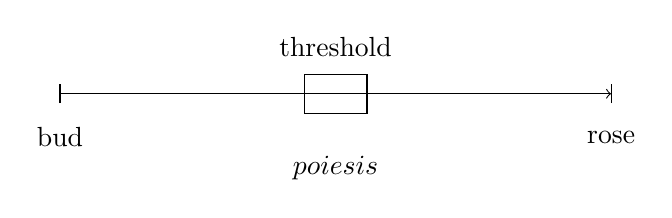
\begin{tikzpicture}
\draw[->] (0,0) -- (7,0);
\draw (0,-0.12) -- (0,0.12);
\draw (7,-0.12) -- (7,0.12);
\draw (3.1,-0.25) rectangle (3.9,0.25);
\node at (0,-0.55) {bud};
\node at (7,-0.55) {rose};
\node at (3.5,0.6) {threshold};
\node at (3.5,-0.95) {$\text{poiesis}$};
\end{tikzpicture}
\end{center}
\end{figure}

The host's analogy to film editing and frame-by-frame slowing belongs here as well. If we zoom deeply enough into a process, what looked like one named state reveals multiple stages. The same is true of perception. To write well, we often have to slow the world until its intermediate states become legible.

\subsection{Question \& Answer}

Is a subject cliche in itself, or only when we fail to estrange it?

In this lecture, the subject is not the problem. The treatment is the problem. A writer fails when the object remains trapped in its ready-made social label. A writer succeeds when the object is displaced, re-entered, or brought into a threshold where perception wakes up again. The practical consequences are direct:
\begin{enumerate}
\item Do not ban the familiar object.
\item Refuse the first available treatment of that object.
\item Reposition, rename, or re-time it.
\item Keep writing until recognition becomes seeing.
\end{enumerate}

\section{Syntax, Haunting, and the Pattern Logic of Reading}

The lecture now moves from the object to the reader. How does a sentence lodge in us? Vuong's answer begins with a proportion that is deliberately rough:
\begin{equation}
80\% \ \text{looking and thinking}, \qquad 20\% \ \text{syntax}.
\end{equation}
He immediately qualifies it: the final twenty percent is everything, because syntax is the downloading mechanism. Perception supplies the material, but syntax is how the material enters the nervous system of the reader.

So the lecture's next schematic is:
\begin{equation}
\text{perception} + \text{syntax} \Longrightarrow \text{haunting}.
\end{equation}
Vuong's preferred readerly effect is not capture but afterlife. He is less interested in how to hook a reader than in how to stay with one. Browning's \textit{Meeting at Night} matters here because it persists in memory far beyond paraphrase. It is not merely understood. It is carried.

The Richard Siken example works by the same logic. Stars become "little boats rowed out too far." The metaphor is not only fresh. It shrinks a grand, overused symbol into a lonely human scale. Loss, lateness, distance, and queer historical grief all enter the line without being discursively explained. Ben Lerner's famous classroom Google-test then supplies the pedagogical corollary:
\begin{equation}
\text{good line} \neq \text{already-said line}.
\end{equation}
A line may be competent and still be one that hundreds of thousands have already written. The bar, in Vuong's account, is higher.

The same issue appears in the host's example from \textit{Good Will Hunting}. A flat abstraction about experience and love could have delivered the information, but the scene becomes memorable only when it moves into vulnerable, image-rich syntax. At that point the reader is no longer merely told something true. The reader feels the truth becoming pressurized.

This leads naturally to the lecture's most general model of linear art:
\begin{equation}
\text{pattern} \Longrightarrow \text{either satisfy expectation or deny expectation}.
\end{equation}
Because prose unfolds in sequence, it creates anticipations. Music does this. Film editing does this. DJ structure does this. Street-ball performance and skate videos do this. Once expectation exists, the maker has two principal resources:
\begin{equation}
\text{satisfy/deny expectation} \Longrightarrow \text{delight} + \text{surprise} + \text{estrangement}.
\end{equation}
This is why Vuong can move so easily from literature to beat drops, deceptive dribbling, and the timing of a trick. The underlying logic is shared. The reader experiences exhilaration when the work seems to know the expectation better than the reader does.

\paragraph{Pattern Rule.}
\begin{enumerate}
\item A sentence unfolds in time and therefore generates expectation.
\item Syntax can confirm that expectation or suspend it.
\item Suspension intensifies attention because the reader senses withheld completion.
\item When completion finally comes, or is denied at the right moment, the sentence acquires residue.
\item That residue is what the lecture calls haunting.
\end{enumerate}

\subsection{Question \& Answer}

How does a sentence stay with a reader rather than merely hook one?

A hook seizes attention for the moment. Haunting survives the moment. In Vuong's account, a sentence stays when perception and syntax are fused so tightly that the line cannot be reduced to information. The sentence must carry rhythm, delay, and emotional pressure. That is why the lecture keeps returning to the difference between abstract statement and embodied phrasing. We remember the line that changes our internal tempo.

\section{Poetry and Nature Writing as Laboratories of Language}

From readerly effect the lecture moves into a broader theory of artistic formation. Poetry matters here not because it is nobler than prose, but because it removes obligations. One need not maintain plot, scene-management, or explanatory throughput at every instant. The sentence is allowed to experiment.

Vuong's compact formula is:
\begin{equation}
\text{assignment removed} \Longrightarrow \text{language becomes available for experiment}.
\end{equation}
From this follows a broader claim:
\begin{equation}
\text{poetry},\ \text{nature writing} \Longrightarrow \text{highest local freedom for the sentence}.
\end{equation}
Poetry is the obvious laboratory because it can attend to language itself. Nature writing becomes a second laboratory for the opposite reason: if it remains purely mimetic, it collapses. We have already seen the meadow. We know what mud looks like. We do not need a sentence that merely duplicates available sight.

This is why J.A. Baker becomes such a decisive example. Baker begins with ordinary weather and marsh description, then moves into a proliferating mud-syntax that no longer merely names substance. Mud becomes texture, pressure, threat, clinging element, psychic atmosphere. By the end, the lecture insists, Baker is no longer only describing mud. He has allowed interiority to enter the description. The mimetic dam has broken:
\begin{equation}
\text{mud description} + \text{released interiority} \Longrightarrow \text{mimesis broken}.
\end{equation}

The host's language of fun belongs to the same argument. The laboratory is not opposed to rigor. It is rigor without premature closure. The delight of seeing that Crayola has many blues is structurally similar to the delight of discovering that mud has more states than one name suggests. Childlike perception is not childishness. It is resistance to dead naming.

Eduardo C. Corral's moss-and-applause simile gives the lecture one more technical refinement. Here the correspondence is not visual. Vuong stresses that the comparison succeeds by behavior:
\begin{align}
\text{applause} \not\sim \text{moss by image}, \qquad \text{applause} \sim \text{moss by behavior},\\
\text{behavioral correspondence} \Longrightarrow \text{apparent acceleration of moss growth}.
\end{align}

\paragraph{Worked Example: Moss and Applause.}
\begin{enumerate}
\item We reject the easy question, "what does moss look like?"
\item We ask instead, "how does moss behave?"
\item Applause offers a model of spread, pulse, quickening, and diffuse collective motion.
\item That borrowed behavior is transferred to moss.
\item The reader now seems to see moss growing faster, even though moss is usually imperceptibly slow.
\item The metaphor therefore changes temporal experience, just as Babel's sunset did.
\end{enumerate}

The anecdote that Corral spent nine years on a short book matters because it returns us to the lecture's opening premise: strong metaphor is often the product of long looking, not sudden cleverness.

\subsection{Question \& Answer}

Why do poetry and nature writing preserve freedom for the sentence better than most contemporary prose?

Because both forms can relax the pressure of assignment. In poetry there need be no plot-duty at all. In nature writing, mere report is inadequate from the start, since the reader already has access to the visible object. Both forms therefore force the writer toward subjective re-seeing. The laboratory is simply the place where the sentence is permitted to discover more than one use for the world.

\section{Publishing Time, Reader Time, and the Ethics of Daringness}

The lecture's last movement gathers institutional critique, readerly temporality, word-use, and artistic ethics into one frame. Vuong has already argued that house styles, editors, software, and classrooms can flatten language. Now he explains why the system so often rewards this flattening. The key theoretical tool comes from Uri Lotman.

\begin{definition}
Lotman's two-time model of reading is
\begin{equation}
\text{reading} = (\text{synchronic line},\text{diachronic line}).
\end{equation}
A synchronic reading places the work in its immediate season, market, publicity cycle, and contemporary institution. A diachronic reading places the work against the longer time of other books, older forms, and accumulated memory.
\end{definition}

Hence the lecture's institutional diagnosis:
\begin{equation}
\text{system judges synchronically}, \qquad \text{reader judges diachronically}.
\end{equation}
Publishing works in seasons. Review culture works in seasons. Prize culture works in seasons. A reader does not. A reader may have been reading Melville last week, Baldwin yesterday, Shakespeare years ago, and a current novel this morning. The reader's standard is not the curated shelf of one season. It is the long carried archive of experience.

\paragraph{A transcript-backed schematic.}
\begin{figure}
\begin{center}
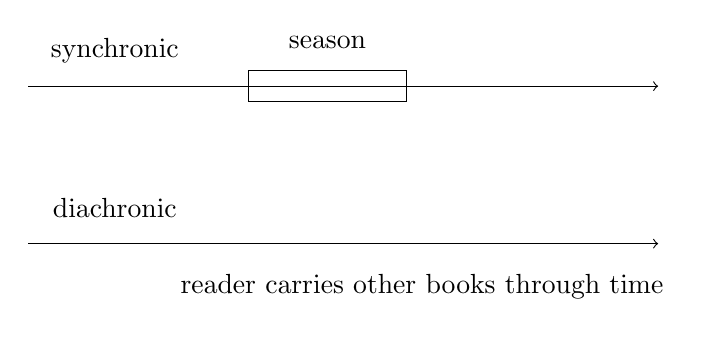
\begin{tikzpicture}
\draw[->] (0,2) -- (8,2);
\draw[->] (0,0) -- (8,0);
\draw (2.8,1.8) rectangle (4.8,2.2);
\node at (1.1,2.45) {synchronic};
\node at (3.8,2.55) {season};
\node at (1.1,0.45) {diachronic};
\node at (5.0,-0.55) {reader carries other books through time};
\end{tikzpicture}
\end{center}
\end{figure}

This is why a book can be praised all the way through the machinery of production and still fail when it reaches readers. The system has rewarded recognizability within the season. The reader measures the work against a much longer and less manageable scale. The host's Rotten Tomatoes analogy belongs here: critic scores often register the institutional moment, while audiences register a different, more distributed life of comparison.

Vuong's anecdote about the "reader in the Midwest" is a perfect exposure of the same cynicism. The system imagines a simplified reader in order to justify simplification. Vuong rejects the premise. The ordinary reader, he insists, has a nervous system, memory, and intelligence. One does not honor the reader by thinning the sentence in advance.

The argument then broadens from books to language itself. Wittgenstein provides the rule:
\begin{equation}
\text{meaning of a word} = \text{its use}.
\end{equation}
The dictionary does not govern use from above. It trails living usage. This matters for Vuong's bilingual reflections, for slang, for etymology, and for the teaching of writing. A student intimidated by the dictionary must be reminded that new forms of use continually reshape the language. The margin is not a decorative edge. It is where linguistic mobility is strongest.

That principle feeds directly into the lecture's concentric model of culture:
\begin{equation}
\text{innovation on margins} \Longrightarrow \text{capture by center} \Longrightarrow \text{homogenized product}.
\end{equation}
The margin invents. The center commercializes. The result is recognition without force. This is why Vuong pairs daringness with disobedience. Daringness is the willingness to risk the failure of innovation. Disobedience is the refusal to obey inherited commands merely because they are inherited.

The skateboarding analogy makes the ethic concrete. One throws oneself toward a trick without any guarantee of landing it. Sometimes there is success. Sometimes there is only bruising. Yet the practice itself teaches a relation to failure, risk, body, timing, and communal delight. Writing, in this late lecture, belongs to the same moral field.

The last question pushes beyond aesthetics. Language has made Vuong's life. It has given livelihood, intellectual power, and enlargement of perception. But language is also an instrument of domination. Newspapers can be captured. Radio can be captured. Tyrannies do not despise language; they seize it first. The lecture therefore closes with an unresolved pair:
\begin{align}
\text{language} &\Longrightarrow \text{power} + \text{livelihood} + \text{enlarged perception},\\
\text{language} &\Longrightarrow \text{capture} + \text{tyranny} + \text{homogenization}.
\end{align}
The historical examples sharpen the paradox rather than soften it. A slaver can keep a library. Cultured men can read great poetry and still commit atrocity. Yet literature can also alter history. Vuong refuses both sentimental certainty and easy despair. The page remains a site of real magic, but not of guaranteed redemption.

\subsection{Question \& Answer}

Why does the culture ask for originality and then reward conformity, and what is a writer supposed to do about it?

Because institutions monetize recognizability. A house style is easier to edit, easier to brand, easier to sell, and easier to praise on schedule. Originality is admired in retrospect but often punished in process. The writer's answer, in Vuong's account, is not a fantasy of pure escape. It is a discipline:
\begin{enumerate}
\item protect the original matrix of surprise rather than surrendering it too early,
\item read diachronically rather than only seasonally,
\item trust living use more than official rule,
\item practice daringness and disobedience together,
\item accept that language is powerful without pretending it is innocent.
\end{enumerate}

\section{Summary}

The lecture begins with a small problem and ends with a large one. We start by asking how a metaphor works. We end by asking what language can and cannot save. Between those poles Vuong constructs a continuous argument: metaphor is observation carried through syntax; workshop should recognize rather than prematurely correct; the modern sentence was historically tamed by journalism and standardization; estrangement rescues the familiar by returning us to threshold and process; syntax makes perception linger in the reader; poetry and nature writing preserve experimental freedom; and publishing systems too often judge on a short clock that readers do not inhabit.

What remains at the end is not a program of rules but a posture. We must look longer, distrust the invisible sentence when it becomes merely obedient, and risk the strange line when the world demands it. The lecture's deepest claim is that writing is not the naming of things already known. It is the repeated effort to make consciousness, through language, see again.